\chapter{Basic models for solid state}
\label{ChapBasicModels}

Many properties of solids can be understood using one-electron models, that is, non-interacting models. When the interaction between the ions and the valence electrons can be mostly neglected one can adapt the free electron approximation. This model is mostly limited to the study of metals and despite its simplicity it successfully explains phenomena related with electrical conductivity and heat capacity. In the opposite limit, we can consider systems in which the ion potential is so large that the electrons are bound in the cores with occasional jumps from site to site. This is known as tight binding model and it can be used to study a wide variety of solids. It is typically used for calculations of the electronic band structure.

Despite the success of the single particle models, there are several phenomena which cannot be explained neglecting electron correlations. For example, high temperature superconductivity cannot be understood with these models. The Hubbard model is the simplest model including electron correlations and despite its simplicity it is not fully understood yet. In this Chapter we will outline the main features of the tight binding model and the Hubbard model, which are basic tools for any condensed matter researcher.

\section{Tight binding}

When the electrons are strongly localized in the atom cores, the wavefunction describing such an electron is similar to the corresponding atomic orbital. Therefore it is natural to consider linear superposition of atomic orbitals as an anstatz for the crystal electron states.

Let the atomic Hamiltonian be $\hat{H}_a(\bs{r}) = -\frac{\hbar^2\hat{p}^2}{2m} + V_a(\bs{r}-\bs{r}_n)$, where $\hbar$ is the reduced Planck constant, $m$ is the electron mass, $\hat{p}$ is the momentum operator and $V_a(\bs{r})$ is the atomic potential. Let $\phi_i(\bs{r})$ be the i-\textit{th} eigenstate of the atomic Hamiltonian with energy $E_i$. The crystal Hamiltonian is:

\begin{equation}
\label{CrystalHam}
\hat{H} = -\frac{\hbar^2p^2}{2m} + \sum_n V_a(\bs{r}-\bs{r}_n)
\end{equation}
An electron localized around the atom at $\bs{r}_n$ will mainly feel the potential of that atom, and the potential of the rest of the atoms will be a perturbation to the free atom problem. That is, we can spit \ref{CrystalHam} into:
\begin{equation}
\label{SplitCrystalHam}
\hat{H} = \hat{H}_a + v(\bs{r}-\bs{r}_n)
\end{equation}
Where $v(\bs{r}-\bs{r}_n) = \sum_{m \neq n} V_a(\bs{r}-\bs{r}_m)$ is a small perturbation. We can expect the crystal electron to retain the properties of the free atom electron, and so, it is natural to describe the crystal electron as a superposition of atomic orbitals. Thus, we will try to find solutions of the form:

\begin{equation}
\psi_i(\bs{r}) = \sum_n b_i(\bs{r}_n) \phi_i(\bs{r}-\bs{r}_n)
\end{equation}
Now, the Bloch theorem states that an eigenfunction of the crystal Hamiltonian should only change by a phase from site to site, that is $\psi_i(\bs{r}+\bs{r}_m)=e^{i \bs{k} \cdot \bs{r}_m}\psi_i(\bs{r})$, where $\bs{k}$ is the crystal momentum of the Bloch wave. We can see that see implies $b_i(\bs{r}_m) = e^{i \bs{k} \cdot \bs{r}_m}b_i(0)$, by normalizing $\psi_i(\bs{r})$ we find $b_i(0) = \frac{1}{\sqrt{N}}$, where $N$ is the number of atoms in the crystal. We therefore obtain:

\begin{equation}
\psi_{i\bs{k}}(\bs{r}) = \frac{1}{\sqrt{N}}\sum_n  e^{i \bs{k} \cdot \bs{r}_n} \phi_i(\bs{r}-\bs{r}_n)
\end{equation}
The energy of this state is $E_i(\bs{k}) = \bra{\psi_{i\bs{k}}} \hat{H} \ket{\psi_{i\bs{k}}}$, using \ref{SplitCrystalHam} this can be written as:

\begin{equation}
E_i(\bs{k}) = \frac{1}{N} \sum_{n,m} e^{i\bs{k}\cdot(\bs{r}_n-\bs{r}_m)} \int \phi_i^*(\bs{r}-\bs{r}_m) (E_i+v(\bs{r}-\bs{r}_n)) \phi_i(\bs{r}-\bs{r}_n) d\bs{r}
\end{equation}
Assuming that $\phi_i$ is spherically symmetric, and neglecting the perturbation $v(\bs{r}-\bs{r}_n)$ further away than nearest neighbors, we can simplify this expression to:

\begin{equation}
\label{TBBand}
E_i(\bs{k}) = E_i - A - B\sum_{\bs{\delta}} e^{i\bs{k}\cdot \bs{\delta}}
\end{equation}
Where $\bs{\delta}$ are the NN vectors and:
\begin{align*}
A &= -\bra{\phi_i(\bs{r}-\bs{r}_n)}v(\bs{r}-\bs{r}_n) \ket{\phi_i(\bs{r}-\bs{r}_n)} \\
B &= -\bra{\phi_i(\bs{r}-\bs{r}_m)}v(\bs{r}-\bs{r}_n) \ket{\phi_i(\bs{r}-\bs{r}_n)}
\end{align*}
$A$ measures the amount of energy reduced when the atom forms a crystal, $B$ is a measure of the width of the band. 
In second quantization formalism we can write the tight binding single band Hamiltonian as:

\begin{equation}
\label{TBModel}
\hat{H} = -t\sum_{\langle i,j \rangle \sigma} \hat{c}^{\dagger}_{i\sigma}\hat{c}_{j\sigma}
\end{equation}
Where $\hat{c}^{\dagger}_{i\sigma}$ ($\hat{c}_{i\sigma}$) creates (annihilates) an electron in site $i$ and spin state $\sigma$. The quantity $t$ is the hopping amplitude, and plays the same role $B$ in the first quantization formalism. We can obtain back \ref{TBBand} by changing basis to momentum space $\hat{c}_{k\sigma} = \frac{1}{\sqrt{N}}\sum_j e^{-i\bs{k}\cdot\bs{r}_j}\hat{c}_{j\sigma}$. In Appendix \ref{APD} we use this formalism to compute the band structure of a two dimensional system in a honeycomb lattice (i.e. graphene).



\section{The Hubbard model}

As we discuss earlier, even tough the tight binding model is successful in describing the band structure of most solids, it fails in some cases. In strongly correlated electron systems, the effect of electron-electron Coulomb interactions is important, and this effect is neglected in \ref{TBModel}. The simplest way to take this effect into account is to consider the interaction of electrons in the same site only, that is, adding a term of the form $\text{U}\sum_i \hat{n}_{i\uparrow}\hat{n}_{i\downarrow}$, where $\text{U}$ is a constant accounting for the onsite electron-electron interaction:
\begin{equation}
\label{HH}
\hat{H} = -t\sum_{\langle i,j \rangle \sigma} \hat{c}^{\dagger}_{i\sigma}\hat{c}_{j\sigma} + \text{U}\sum_i \hat{n}_{i\uparrow}\hat{n}_{i\downarrow}
\end{equation}
This is known as the Hubbard model, which was first proposed by Hubbard \cite{Hubbard1963} to describe electron correlations in $d$ or $f$ bands in transition metals. The result was a simplified model to predict metal-insulator transitions. However, it exhibits much richer phenomena. It can be considered an impoved tight binding model, describing Mott insulators, which cannot be describied by band theory (i.e. they should be conductors according to band theory, but electron-electron interactions keep away from). Also, the attractive Hubbard model (where $\text{U} < 0$) can be considered an effective model relevant for understanding high temperature superconductivity \cite{Alexandrov1981}. Despite its simplicity the ground state has no analytic form in more than one dimensions, and different computational methods must be used to study it.

 Figure \ref{fig:Hubbard} shows a graphical representation of the parameters in \ref{HH}. The new term $\text{U}\sum_i \hat{n}_{i\uparrow}\hat{n}_{i\downarrow}$ will add an energy $+\text{U}$ when a site is double occupied ($\hat{n}_{i\uparrow} = \hat{n}_{i\downarrow} = 1$) and will not contribute in the more normal case, that $\hat{n}_{i\uparrow} + \hat{n}_{i\downarrow} = 1$. The half-filled case is most commonly studied, this is the situation where the system has one electron per site (or it has half the maximum allowed number). This situation is simpler in many ways and it exhibits a lot of interesting phenomena (Mott insulating behavior, antiferromagnetic order, etc.). However, other cases have also been widely studied.

\begin{figure}
\centering
  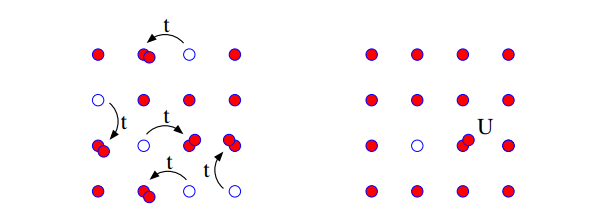
\includegraphics[width=\linewidth]{../Figures/hubbard.png}
  \caption{Image from Scalettar's notes representing the kinetic term $t$ and the on-site interaction $\text{U}$ in the Hubbard model.} 
\label{fig:Hubbard}
\end{figure}
Notice that if we set $\text{U}=0$ in \ref{HH} we recover the tight binding Hamiltonian, therefore we can say that the Hubbard model is an expansion of the tight binding model. The opposite limit $t=0$ is more interesting. In the half-filling case, for $\text{U}>0$ the ground state will be any state with exactly one electron per site. Since each electron can be in two spin states there is a $2^N$ degeneracy. The subspace spanned by these states is referred to as low energy subspace, and in this case is has energy $E_0 = 0$. If we switch $0 \neq t \ll \text{U}$ this hopping term will allow an even further decrease in energy by allowing virtual processes $i \rightarrow j \rightarrow i$ that localized the electrons withing their neighbor sites. For $t \ll \text{U}$ the dynamics of the system can be described withing the low energy subspace only, by doing so we can obtain an effective spin Hamiltonian $\hat{H}_{\text{eff}} = \sum{\langle i,j \rangle} J \bs{S}_i\cdot\bs{S}_j$ where $J>0$ describing an antiferromagnetic system. A rigorous derivation of this will be offered in the next Chapter, however we can intuitively understand this result in the following way: the virtual processes $i \rightarrow j \rightarrow i$ will be allowed when the electrons at sites $i$ and $j$ have opposite spin (otherwise it would contradict the Pauli principle), therefore states where neighbor sites have opposite spins will have a lower energy due to the delocalization mechanism. Additionally, the constant $J$ will be proportional to the amplitude of the process $i \rightarrow j \rightarrow i$. We can already see that this amplitude is $2\frac{t^2}{\text{U}}$, $t^2$ due to two hopping processes, $\frac{1}{\text{U}}$ due to the energy of the intermediate state and the factor $2$ due to the two spin possibilities.

In the next Chapter and in the rest of this thesis we will consider the effects of spin orbit interaction (SOI) in strongly correlated systems. For this reason we will have an additionally spin dependent hopping term in \ref{HH} arising from the SOI. This additional term will lead to a DMI when deriving the effective spin Hamiltonian in the $t \ll \text{U}$ limit.






